\section{Introduction}\label{sec:intro}
EDB is short for External Data Broker and EDB FMU is an FMU that brings external
data into an FMI context. The implementation of EDB FMU described in this
publication is based on RabbitMQ. However, this is just one way to implement an
EDB FMU. Several of the constructs described in this publication are general and
can be used with other message-oriented or data streaming middleware. For this
reason, both EDB FMU and RabbitMQ FMU will be used throughout this document,
where EDB FMU is generally applicable functionality, whereas RabbitMQ FMU is an
implementation of EDB FMU specific to RabbitMQ. Thus, one could take the
existing source code of RabbitMQ FMU and fit it to another middleware than
RabbitMQ while still reusing most of the source code.
Note, that this document assumes general knowledge of
the Functional Mock-up Interface (FMI)~\cite{FMIStandard2.1}.

An overall approach to using an EDB FMU in a digital twin context is depicted
in~\cref{fig:interfacing_overview}, where the content within the \textit{System Specific} frame will vary based on the system
providing the data. The Log-Translator entity translates the
system-specific log messages to digital twin compatible messages and publishes
them to a Data Middleware Node (i.e. a RabbitMQ Node). The EDB FMU is configured
via its static description to
receives messages from the Data Middleware Node. The message content is then
parsed and published via regular FMI outputs.

\begin{figure}[htb]
  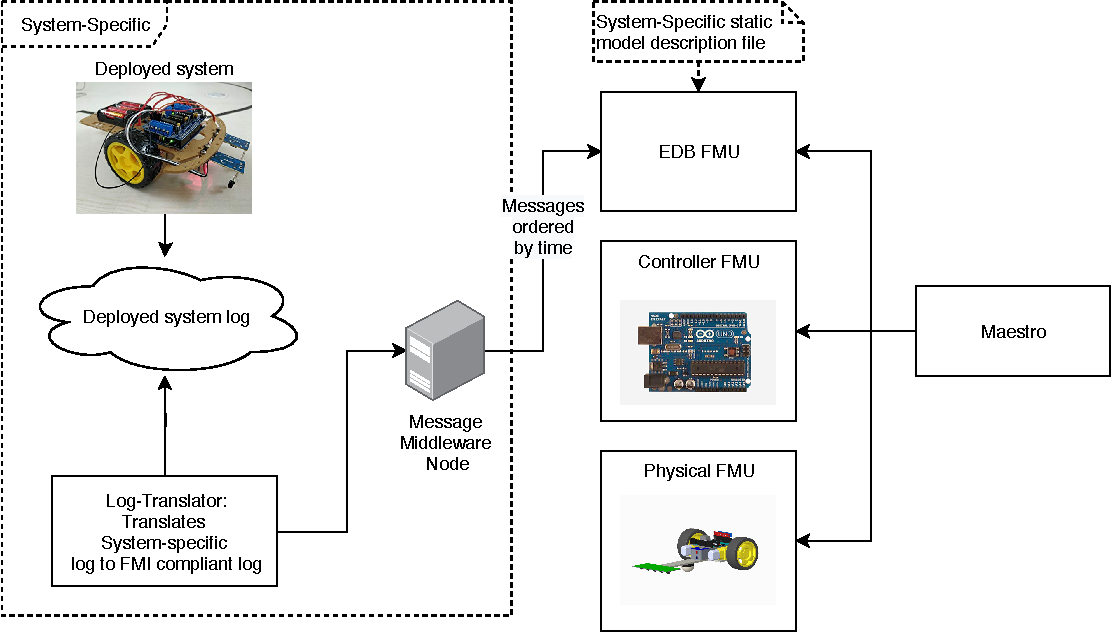
\includegraphics[width=\textwidth]{figures/overview.pdf}
  \caption{Interfacing Overview}
 \label{fig:interfacing_overview}
\end{figure}

This approach generalises the FMI enabling entity, the EDB FMU, such that
it can be used for different kinds of systems with different kinds of logging
facilities. The motivation behind this approach is that tools of the INTO-CPS Association
should be generally applicable.

The following chapters describes the following in order:
\begin{description}
  \item[Time Handling] How system-time and simulation time is mapped and put in
    an FMI simulation context.
  \item[Data Handling] How message content and the state of EDB FMU are
    coordinated.
  \item[Configuration] How to configure an EDB/RabbitMQ FMU via the ModelDescription File
  \item[Example - Single Water Tank RabbitMQ] This example demonstrates how RabbitMQ FMU
    acts as an External Data Broker in context of a Single Water Tank Digital Twin. It focuses solely on this part and does not
    contain a deployed system.

    \item[Example - Line Following Robot] IN PROGRESS - This example demonstrates transmission
    of data from a deployed line following robot. The data is made available in
    the FMI co-simulatino via RabbitMQ FMU. Thus, this is a example with
    both a deployed system, its digital twin and the RabbitMQ FMU.
  \item[Future Work] Describes some ideas for future work.
\end{description}


%%% Local Variables:
%%% mode: latex
%%% TeX-master: "../rabbitmq-fmu"
%%% End:
